\documentclass[a4paper, 14pt]{extarticle}

% Поля
%--------------------------------------
\usepackage{geometry}
\geometry{a4paper,tmargin=2cm,bmargin=2cm,lmargin=3cm,rmargin=1cm}
%--------------------------------------


%Russian-specific packages
%--------------------------------------
\usepackage[T2A]{fontenc}
\usepackage[utf8]{inputenc} 
\usepackage[english, main=russian]{babel}
%--------------------------------------

\usepackage{textcomp}

% Красная строка
%--------------------------------------
\usepackage{indentfirst}               
%--------------------------------------             


%Graphics
%--------------------------------------
\usepackage{graphicx}
\graphicspath{ {./images/} }
\usepackage{wrapfig}
%--------------------------------------

% Полуторный интервал
%--------------------------------------
\linespread{1.3}                    
%--------------------------------------

%Выравнивание и переносы
%--------------------------------------
% Избавляемся от переполнений
\sloppy
% Запрещаем разрыв страницы после первой строки абзаца
\clubpenalty=10000
% Запрещаем разрыв страницы после последней строки абзаца
\widowpenalty=10000
%--------------------------------------

%Списки
\usepackage{enumitem}

%Подписи
\usepackage{caption} 

%Гиперссылки
\usepackage{hyperref}

\hypersetup {
	unicode=true
}

%Рисунки
%--------------------------------------
\DeclareCaptionLabelSeparator*{emdash}{~--- }
\captionsetup[figure]{labelsep=emdash,font=onehalfspacing,position=bottom}
%--------------------------------------

\usepackage{tempora}

%Листинги
%--------------------------------------
\usepackage{listings}
\lstset{
  basicstyle=\ttfamily\footnotesize, 
  %basicstyle=\footnotesize\AnkaCoder,        % the size of the fonts that are used for the code
  breakatwhitespace=false,         % sets if automatic breaks shoulbd only happen at whitespace
  breaklines=true,                 % sets automatic line breaking
  captionpos=t,                    % sets the caption-position to bottom
  inputencoding=utf8,
  frame=single,                    % adds a frame around the code
  keepspaces=true,                 % keeps spaces in text, useful for keeping indentation of code (possibly needs columns=flexible)
  keywordstyle=\bf,       % keyword style
  numbers=left,                    % where to put the line-numbers; possible values are (none, left, right)
  numbersep=5pt,                   % how far the line-numbers are from the code
  xleftmargin=25pt,
  xrightmargin=25pt,
  showspaces=false,                % show spaces everywhere adding particular underscores; it overrides 'showstringspaces'
  showstringspaces=false,          % underline spaces within strings only
  showtabs=false,                  % show tabs within strings adding particular underscores
  stepnumber=1,                    % the step between two line-numbers. If it's 1, each line will be numbered
  tabsize=2,                       % sets default tabsize to 8 spaces
  title=\lstname                   % show the filename of files included with \lstinputlisting; also try caption instead of title
}
%--------------------------------------

%%% Математические пакеты %%%
%--------------------------------------
\usepackage{amsthm,amsfonts,amsmath,amssymb,amscd}  % Математические дополнения от AMS
\usepackage{mathtools}                              % Добавляет окружение multlined
\usepackage[perpage]{footmisc}
%--------------------------------------

%--------------------------------------
%			НАЧАЛО ДОКУМЕНТА
%--------------------------------------

\begin{document}

%--------------------------------------
%			ТИТУЛЬНЫЙ ЛИСТ
%--------------------------------------
\begin{titlepage}
\thispagestyle{empty}
\newpage


%Шапка титульного листа
%--------------------------------------
\vspace*{-60pt}
\hspace{-65pt}
\begin{minipage}{0.3\textwidth}
\hspace*{-20pt}\centering

\includegraphics[width=\textwidth]{emblem}
\end{minipage}
\begin{minipage}{0.67\textwidth}\small \textbf{
\vspace*{-0.7ex}
\hspace*{-6pt}\centerline{Министерство науки и высшего образования Российской Федерации}
\vspace*{-0.7ex}
\centerline{Федеральное государственное бюджетное образовательное учреждение }
\vspace*{-0.7ex}
\centerline{высшего образования}
\vspace*{-0.7ex}
\centerline{<<Московский государственный технический университет}
\vspace*{-0.7ex}
\centerline{имени Н.Э. Баумана}
\vspace*{-0.7ex}
\centerline{(национальный исследовательский университет)>>}
\vspace*{-0.7ex}
\centerline{(МГТУ им. Н.Э. Баумана)}}
\end{minipage}
%--------------------------------------

%Полосы
%--------------------------------------
\vspace{-25pt}
\hspace{-35pt}\rule{\textwidth}{2.3pt}

\vspace*{-20.3pt}
\hspace{-35pt}\rule{\textwidth}{0.4pt}
%--------------------------------------

\vspace{1.5ex}
\hspace{-35pt} \noindent \small ФАКУЛЬТЕТ\hspace{80pt} <<Информатика и системы управления>>

\vspace*{-16pt}
\hspace{47pt}\rule{0.83\textwidth}{0.4pt}

\vspace{0.5ex}
\hspace{-35pt} \noindent \small КАФЕДРА\hspace{50pt} <<Теоретическая информатика и компьютерные технологии>>

\vspace*{-16pt}
\hspace{30pt}\rule{0.866\textwidth}{0.4pt}
  
\vspace{11em}

\begin{center}
\Large {\bf Лабораторная работа № 2а} \\ 
\large {\bf по курсу <<Языки и методы программирования>>} \\
\large <<Модель вселенной>> 
\end{center}\normalsize

\vspace{8em}


\begin{flushright}
  {Студент группы ИУ9-21Б Горбунов А. Д. \hspace*{15pt}\\ 
  \vspace{2ex}
  Преподаватель Посевин Д. П.\hspace*{15pt}}
\end{flushright}

\bigskip

\vfill
 

\begin{center}
\textsl{Москва 2023}
\end{center}
\end{titlepage}
%--------------------------------------
%		КОНЕЦ ТИТУЛЬНОГО ЛИСТА
%--------------------------------------

\renewcommand{\ttdefault}{pcr}

\setlength{\tabcolsep}{3pt}
\newpage
\setcounter{page}{2}

\section{Задание}\label{Sect::task}

Реализовать модель вселенной. Каждый элемент вселенной должен быть объектом
некоего публичного класса, который инициализируется вспомогательным публичным
классом порождающим эту вселенную. При инициализации экземпляров класса частиц
моделируемой вселенной необходимо подсчитывать количество частиц вселенной используя
статичное экземплярное поле защищенное от изменения из объектов внешних классов путем
реализации статичного метода. Сформировать исходные данные и определить необходимые
экземплярные поля для хранения состояния объектов частиц вселенной в соответствии с
условием задачи и реализовать расчет. 

Определить расстояние между двумя вселенными

\section{Результаты}\label{Sect::res}

Исходный код программы представлен в листингах~\ref{lst:code1}, ~\ref{lst:code2}, ~\ref{lst:code3}, ~\ref{lst:code4}, ~\ref{lst:code5}.

\begin{figure}[!htb]
\begin{lstlisting}[language={},caption={Нахождение расстояние между двумя вселенными(класс Mine},label={lst:code1}]
import java.util.Scanner;
public class Main {
    private static final int n = 10;
    public static void main(String[] args) {
        Scanner scan = new Scanner(System.in);

        Universe univ1 = new Universe(n);
        univ1.newParticlesUniverse(1,1,1);
        univ1.newParticlesUniverse(2,2,2);
        System.out.println(univ1.getX() +" "+univ1.getY() +" "+univ1.getZ());
        Universe univ2 = new Universe(n);
        univ2.newParticlesUniverse(0,0,0);
        univ2.newParticlesUniverse(-1,-1,-1);
        System.out.println(univ2.getX() +" "+univ2.getY() +" "+univ2.getZ());
        double result = univ1.distanceBetweenUniverses(univ2);
        System.out.println(result);
/////////////////////
        Universe univ3 = new Universe(n);
        univ3.newParticlesUniverse(scan.nextInt(),scan.nextInt(),scan.nextInt());
        univ3.newParticlesUniverse(scan.nextInt(),scan.nextInt(),scan.nextInt());
        System.out.println(univ3.getX() +" "+univ3.getY() +" "+univ3.getZ());

\end{lstlisting}
\end{figure}

\newpage

\begin{figure}[!htb]
\begin{lstlisting}[language={},caption={Нахождение расстояния между двумя вселенными (Класс Maine)(продолжение)},label={lst:code2}]
        Universe univ4 = new Universe(n);
        univ4.newParticlesUniverse(scan.nextInt(),scan.nextInt(),scan.nextInt());
        univ4.newParticlesUniverse(scan.nextInt(),scan.nextInt(),scan.nextInt());
        System.out.println(univ4.getX() +" "+univ4.getY() +" "+univ4.getZ());

        System.out.println(result);
    }
}
\end{lstlisting}
\end{figure}

Результат запуска представлен на рисунке~\ref{fig:picture_1.png}.

\begin{figure}[!htb]
\begin{lstlisting}[language={},caption={Нахождение расстояния между двумя вселенными (Класс Universe)},label={lst:code3}]
import static java.lang.Math.*;
public class Universe {
    private static int number_universes;
    private final int particles;
    private int number_particles_this_universe = 0;
    private double x, y, z;
    Particles_universe[] univ;
    public Universe(int particles)
    {
        number_universes++;
        this.particles = particles;
        univ = new Particles_universe[this.particles];
    }
    private void centerUniverse()
    {
        double sup_x=0, sup_y=0, sup_z=0;
        for(int i = 0;i < number_particles_this_universe;i++)
        {
            sup_x += univ[i].getX();
            sup_y += univ[i].getY();
            sup_z += univ[i].getZ();
        }
        this.x = sup_x/number_particles_this_universe;
        this.y = sup_y/number_particles_this_universe;
        this.z = sup_z/number_particles_this_universe;
    }

\end{lstlisting}
\end{figure}

\begin{figure}[!htb]
\begin{lstlisting}[language={},caption={Нахождение расстояния между двумя вселенными (Класс Universe)(продолжение)},label={lst:code4}]
    public void newParticlesUniverse(double x, double y, double z)
    {
        univ[number_particles_this_universe] = new Particles_universe(x, y, z);
        number_particles_this_universe++;
        centerUniverse();
    }

    public double distanceBetweenUniverses(Universe universal)
    {
        return sqrt(pow(universal.getX()-x,2)+pow(universal.getY()-y,2)+pow(universal.getZ()-z,2));
    }
    
    public double getX()
    {
        return this.x;
    }
    public double getY()
    {
        return this.y;
    }
    public double getZ()
    {
        return this.z;
    }
}
\end{lstlisting}
\end{figure}

\begin{figure}[!htb]
\begin{lstlisting}[language={},caption={Нахождение расстояния между двумя вселенными (Класс Particles)(продолжение)},label={lst:code5}]
public class Particles_universe {
    private static long number_particles_universe;
    private double x, y, z;
    public Particles_universe(double x, double y, double z)
    {
        number_particles_universe++;
        this.x = x;
        this.y = y;
        this.z = z;
    }

    public double getX()
    {
        return this.x;
    }
    public double getY()
    {
        return this.y;
    }
    public double getZ()
    {
        return this.z;
    }
    public long getN()
    {
        return number_particles_universe;
    }
}

\end{lstlisting}
\end{figure}

\begin{figure}[!htb]
	\centering
	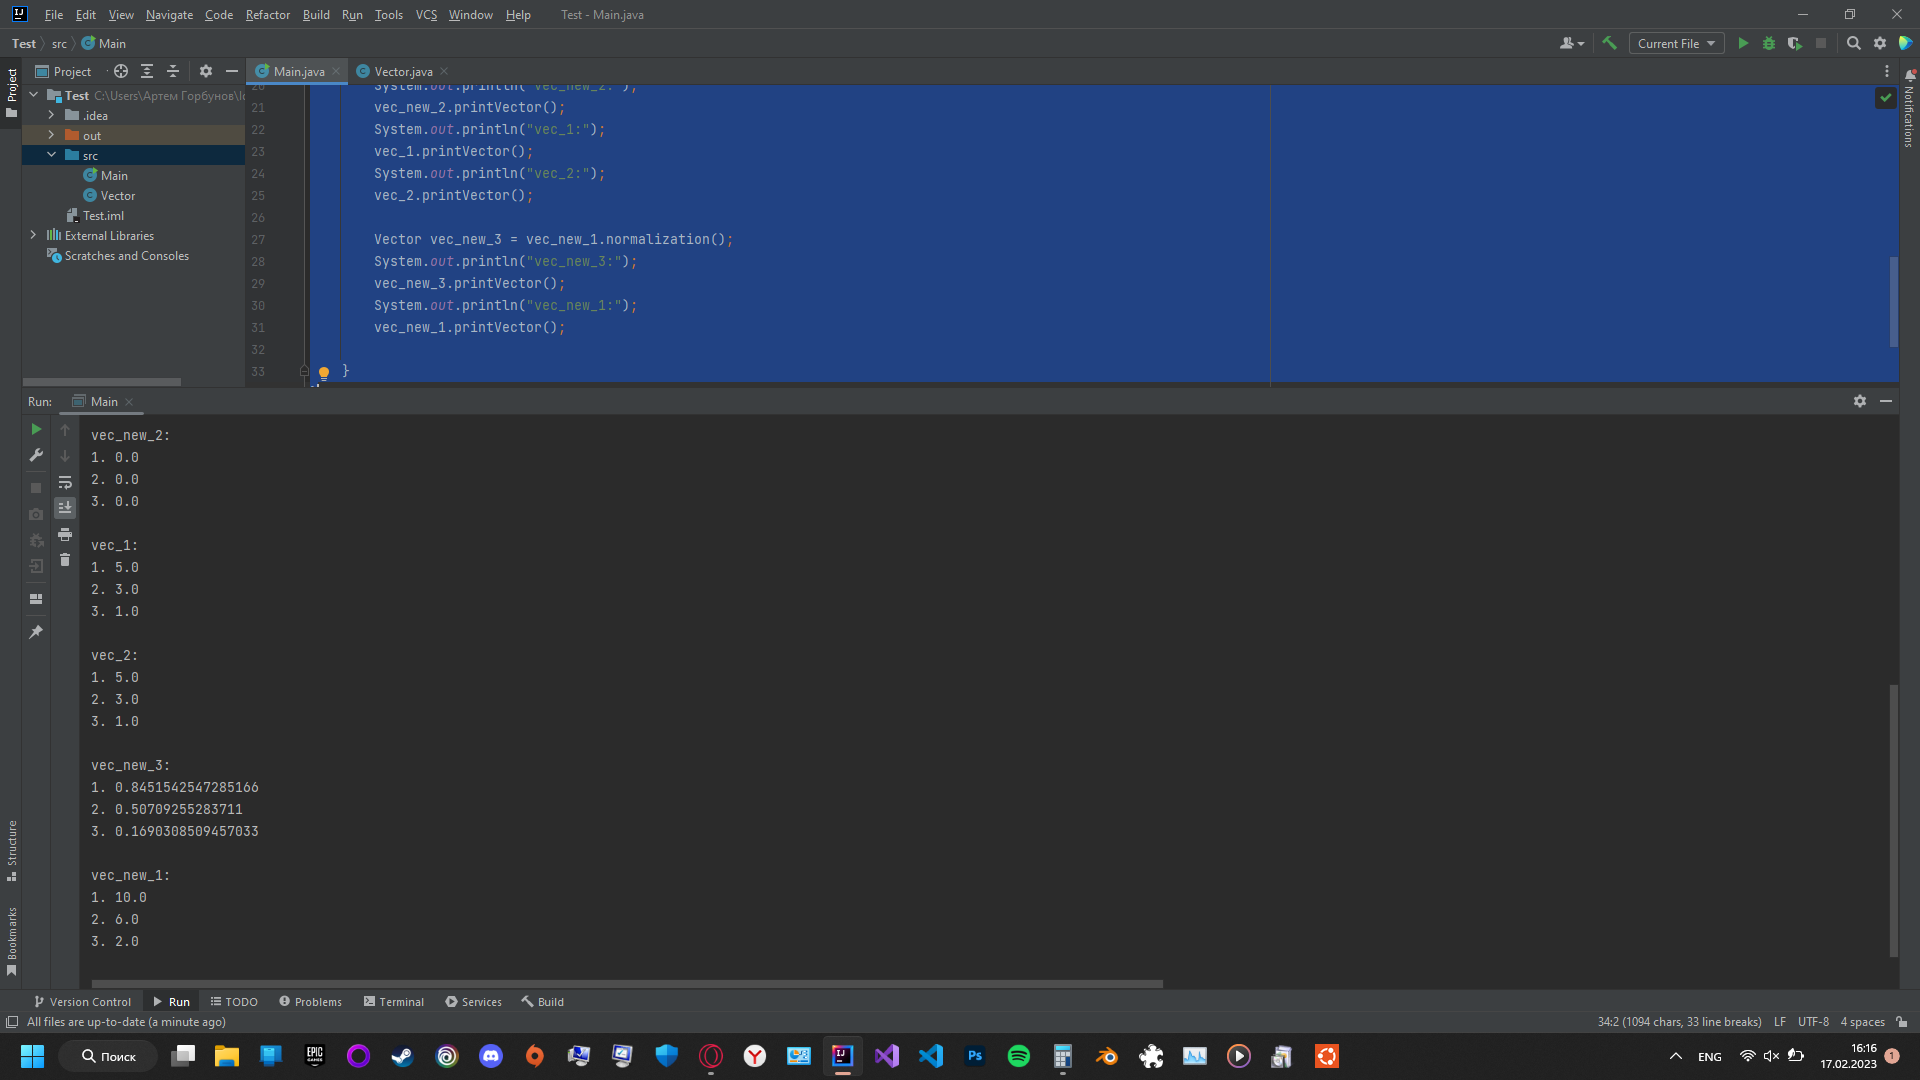
\includegraphics[width=0.8\textwidth]{picture_1.png}
\caption{Вывод программы}
\label{fig:picture_1.png}
\end{figure}

\begin{figure}[!htb]
	\centering
	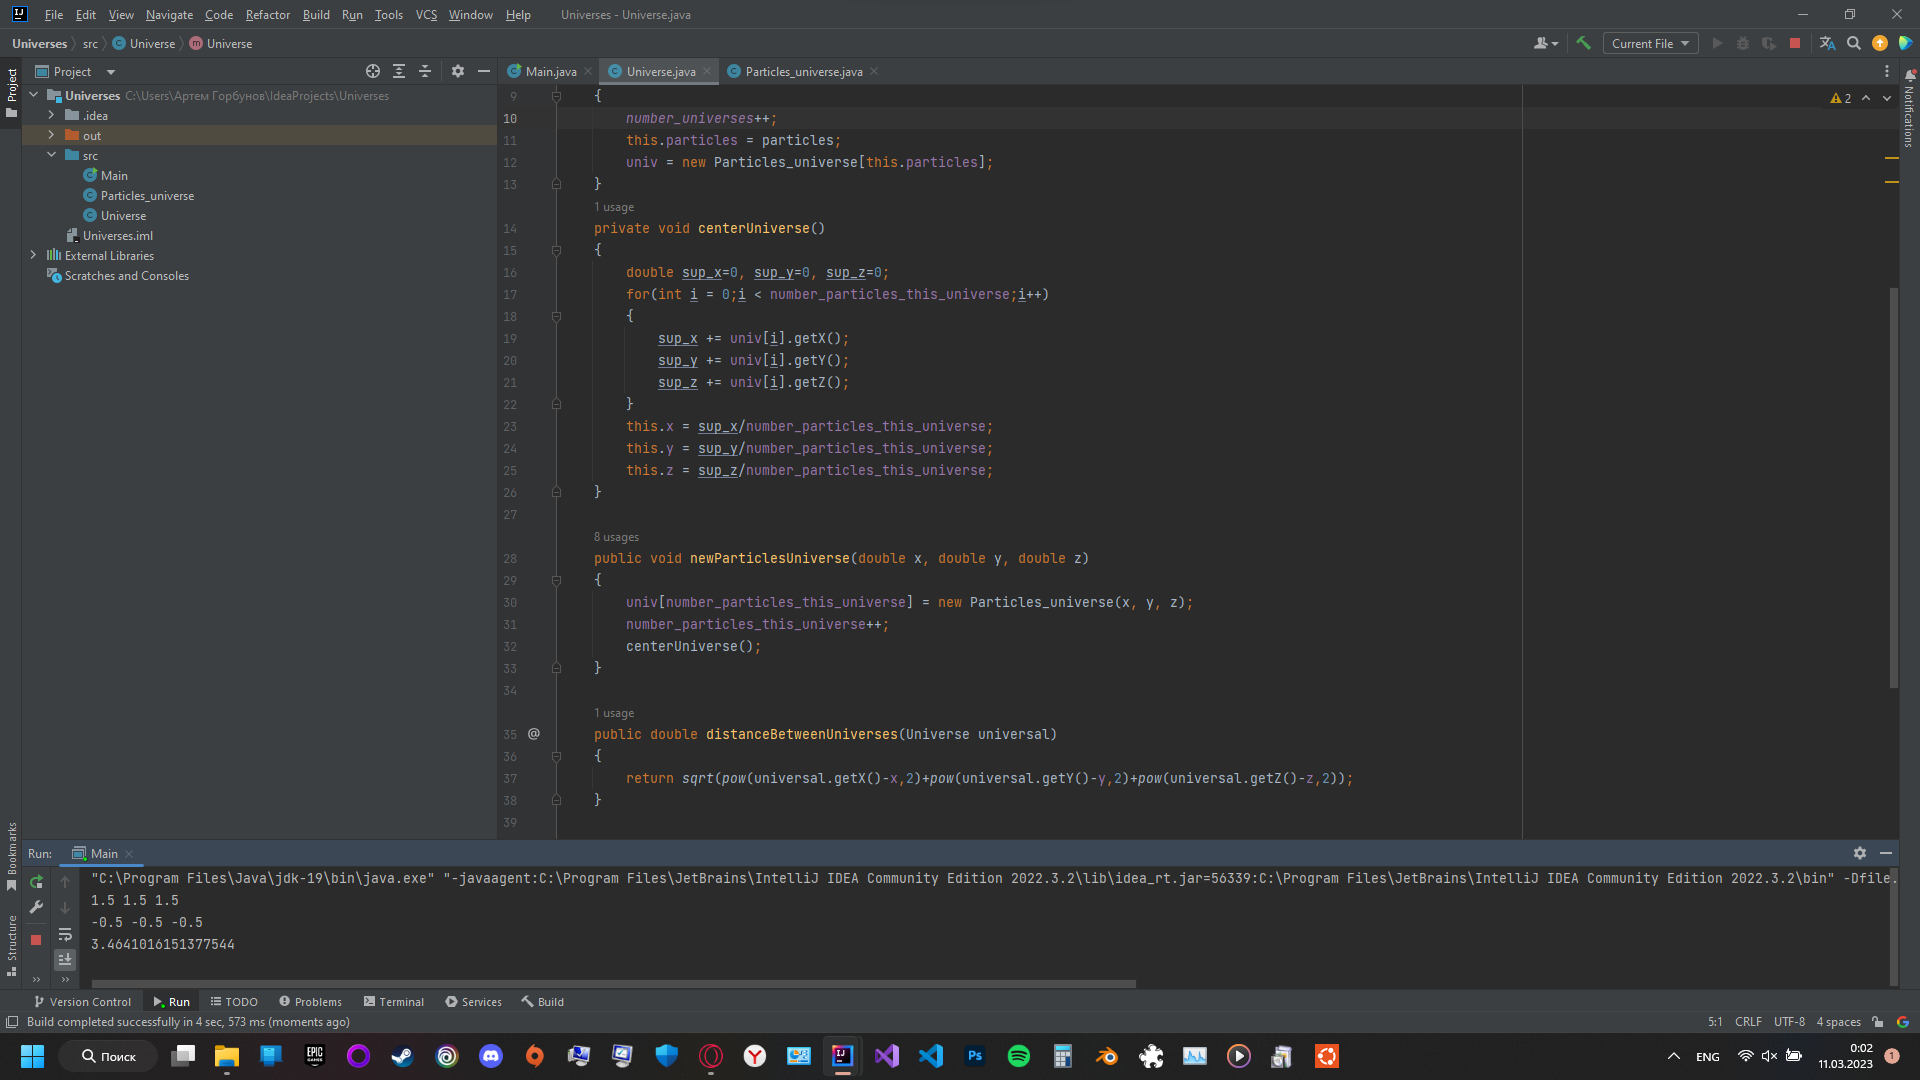
\includegraphics[width=0.8\textwidth]{picture_2.png}
\caption{Работа программы(1)}
\label{fig:picture_2.png}
\end{figure}

\begin{figure}[!htb]
	\centering
	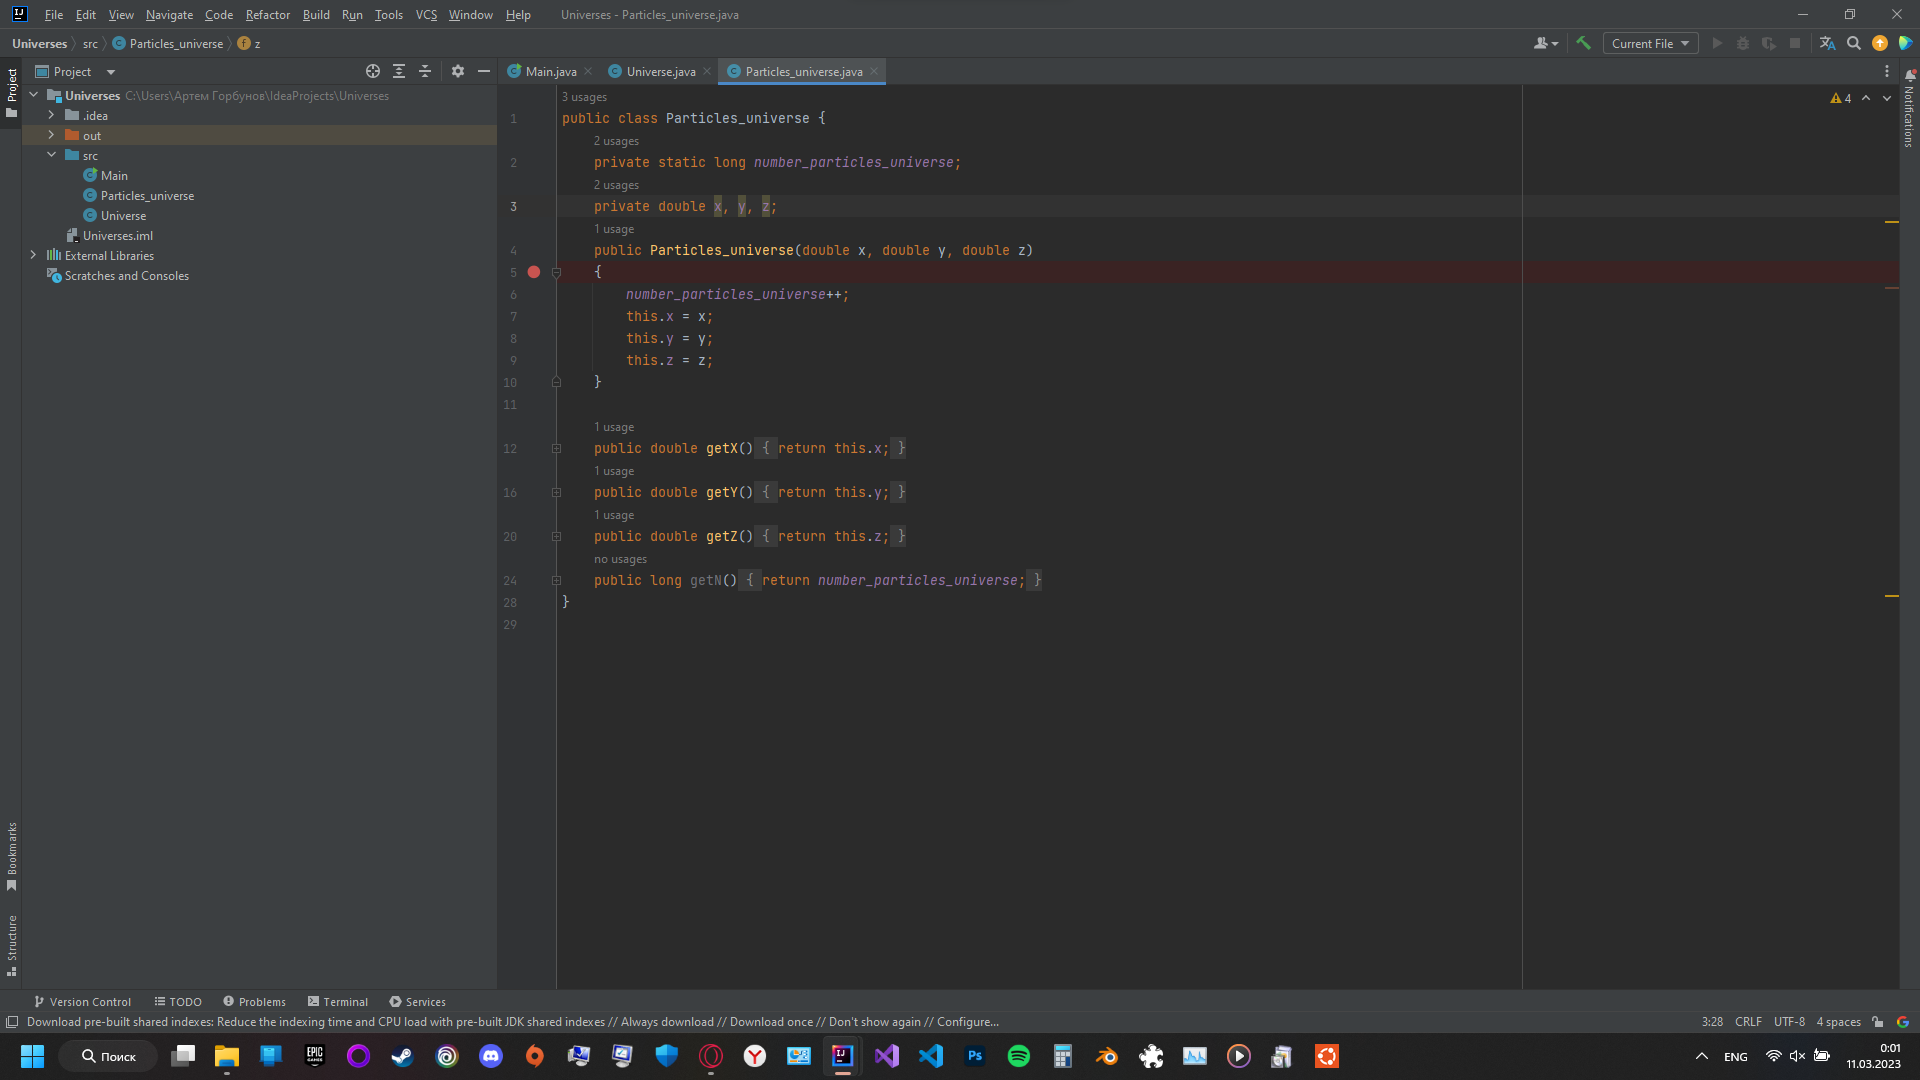
\includegraphics[width=0.8\textwidth]{picture_3.png}
\caption{Работа программы(2)}
\label{fig:picture_3.png}
\end{figure}

\end{document}

